\section{Asynchronmaschine}
\newvideofile{asynchronmaschine}{Asynchronmaschine}
\s{Die Asynchronmaschine ist ebenfalls eine Drehfeldmaschine. Der Stator ist identisch zum Stator der Synchronmaschine, der Rotor ist hingegen in der häufigsten Version dieses Maschinentyps, beim sogenannten Käfigläufer, passiv.}
\begin{frame}\ftx{Asynchronmaschine Aufbau}\index{Asynchronmaschine>Aufbau}\s{\subsection{Aufbau}}
	\fo{width=0.65\textwidth}{height=0.9\textheight}{Aufbau_Asynchron_Kaefig1}{
		\uncover<1->{\put(79,0){\line(-1,1){29.5}}\put(79.2,0){Gehäuse mit Blechpaket}}
		\uncover<3->{\put(79,6){\line(-1,1){27}}\put(79.3,6){Drehstromwicklung}}
		\uncover<2->{\put(90,12){\line(-1,1){40}}\put(90.3,12){Läuferkäfig}}
		\uncover<2->{\put(90,18){\line(-1,1){32}}\put(90.3,18){Blechpaket}}
		\uncover<4->{\put(103,36){\line(-1,1){10}}\put(103.3,36){Flügelhaube}}
		\uncover<4->{\put(103,42){\line(-1,1){27}}\put(103.3,42){Lüfterflügel}}

	}{{\bf Aufbau einer Käfigläufer-Asynchronmaschine.} Die Bleche des Rotorzylinders wurden der Anschaulichkeit halber zur Hälfte beschnitten, um den Käfig freizulegen.}

	\speech{AufbauASM}{1}{Die Asynchronmaschine ist wie die Synchronmaschine eine sogenannte Drehfeldmaschine. Der Stator ist identisch zum Stator der Synchronmaschine, der Rotor ist hingegen in der häufigsten Version dieses Maschinentyps, dem sogenannten Käfigläufer, passiv.}
	\speech{AufbauASM}{2}{Der Rotor besteht aus einem zylindrischen Blechpaket, das mit Kurzschlussstäben, dem sogenannten Läuferkäfig, versehen ist.}
	\speech{AufbauASM}{3}{Der Stator verfügt über die selbe Drehstromwicklung, hier in orange dargestellt, wie die Synchronmaschine.}
	\speech{AufbauASM}{4}{Das Gehäuse verfügt normalerweise über ein angebautes Lüfterrad, das mit der gleichen Drehzahl der Maschine dreht und dafür sorgt, dass die Maschine während des Betriebs gekühlt wird.}
\end{frame}

\begin{frame}\ftb{\index{Käfigläufer}Käfigläufer}
	\begin{itemize}
		\item In den Nuten des Läuferblechpaketes liegen leitfähige Stäbe.
		\item Stirnseitig sind die Stäbe durch Kurzschlussringe miteinander verbunden.
		\item Zusammen bilden diese Komponenten einen Käfig (ähnlich Hamsterkäfig).
		\item Stäbe werden geschrägt ausgeführt zur Reduktion von Oberwellen im umlaufenden magnetischen Feld.
	\end{itemize}
		\f{width=0.5\textwidth}{height=0.6\textheight}{Aufbau_Asynchron_Kaefig2}{{\bf Käfig eines Asynchronrotors.} Zur Hälfte mit Blechpaket gezeigt.}
\end{frame}


\begin{frame}	\ftb{Anlauf der ASM}\index{Asynchronmaschine>Anlauf}
	\begin{itemize}
		\item Der Stator erzeugt im Ständer eine umlaufende magnetische Wanderwelle mit der Winkelgeschwindigkeit:
		$\omega_\mathrm{s} = \frac{\omega_0}{p}$.\pause
		\item Der ruhende Läufer sieht ein veränderliches Feld mit der Frequenz $\omega_\mathrm{s}$.\pause
		\item Das magnetische Drehfeld durchsetzt den Läufer und induziert eine Spannung mit der Frequenz $\omega_\mathrm{s}$.\pause
		\item Aus der Spannungsinduktion resultiert ein Stromfluss, da die Läuferwicklungen kurzgeschlossen sind.\pause
		\item Der induzierte Rotorstrom wirkt der von ihm gesehenen Änderung des Statorfeldes entgegen (Lenzsche Regel).\pause
		\item Statorfeld und Rotorstrom wechselwirken durch die Lorentzkraft- es kommt zur Ausbildung eins Drehmoments.\pause
		\item Das Drehmoment wirkt in Richtung des Ständerdrehfelds.\pause
		\item Der Läufer beginnt sich zu drehen.
	\end{itemize}
\end{frame}

\begin{frame}	\ftb{Betrieb der ASM}    \index{Asynchronmaschine>Funktionsprinzip}
	\begin{itemize}
		\item Mit steigender Drehzahl des Läufers sieht dieser eine immer langsamere Änderung des Statorfeldes:
		$\omega_\mathrm{r} = \omega_\mathrm{s} - \omega_\mathrm{mech}$.\pause
		\item Mit steigender Drehzahl sinkt sowohl der Betrag als auch die Frequenz der induzierten Spannung im Rotor.\pause
		\item Der Betrag des Drehmoments sinkt.\pause
		\item Drehen sich der Läufer und Ständerfeld mit der gleichen Frequenz, ist die synchrone Drehzahl erreicht.\pause
		\item Die Läuferwicklungen sehen keine Änderung des Feldes.\pause
		\item Induzierter Strom und Moment der Maschine werden zu Null.\pause
		\item Durch Reibungseffekte wird der Rotor wieder abgebremst - es kommt zur erneuten Ausbildung eines Moments.\pause
		\item Im Gleichgewichtszustand stellt sich eine Drehzahl knapp unter der synchronen ein.
	\end{itemize}
\end{frame}


\begin{frame}\ftb{Drehzahl/Drehmomenten-Kennlinie}
	\begin{columns}
		\column[c]{0.3\textwidth}
			\b{Schlupf:}
			\s{Die Drehzahl/Drehmomenten-Kennlinie ist bei der Asynchronmaschine nichtlinear und kann in mehrere Abschnitte unterteilt werden. Häufig wird die Kennlinie wie in Abbildung \ref{kloss} gezeigt über den Schlupf $s$ aufgetragen. Der Schlupf\index{Schlupf} bezeichnet die prozentuale Abweichung der mechanischen Drehgeschwindigkeit des Rotors $n_\mathrm{r}$ von der elektrischen Drehgeschwindigkeit $n_\mathrm{s}$ des speisenden Netzes im Stator.}
			\nomenclature[F]{$s$}{Schlupf der Asynchronmaschine}
			\nomenclature[F]{$\omega_\mathrm{s}$}{Synchrone Drehfrequenz des speisenden Netzes \nomunit{$\frac{1}{\mathrm{s}}$}}
			\nomenclature[F]{$\omega_\mathrm{r}$}{Drehfrequenz des Rotors \nomunit{$\frac{1}{\mathrm{s}}$}}
			\begin{eq}
				s = \frac{\omega_\mathrm{s} - \omega_\mathrm{r}}{\omega_\mathrm{s}}
			\end{eq}

			\s{Ein Schlupf von $s=1$ ($100\%$) entspricht daher dem Stillstand der Maschine oder Drehzahl $n=0$, ein Schlupf von $s=0$ entspricht dem netzsynchronen Betrieb, der jedoch bei der Asynchronmaschine niemals auftreten kann, da das Drehmoment in dem Fall Null wird.}

			\uncover<2->{
				\s{Die Drehzahl/Drehmomenten-Kennlinie wird auch als Klosssche Kennlinie bezeichnet und kann durch die Gleichung \ref{GlKloss} ausgedrückt werden:}
				\b{Klosssche Gleichung}
				\begin{eq}
					M = \frac{2\cdot M_\mathrm{K}}{\frac{s_\mathrm{K}}{s} + \frac{s}{s_\mathrm{K}}}\label{GlKloss}
				\end{eq}
				\nomenclature[F]{$s_\mathrm{K}$}{Kippschlupf der Asynchronmaschine}
				\nomenclature[F]{$M_\mathrm{K}$}{Kippmoment der Asynchronmaschine \nomunit{Nm}}
			}
			\uncover<3>{

				\s{Der Schlupf entspricht bei großen Maschinen in sehr guter Näherung den prozentualen Verlusten der Maschine:}
				\b{Schlupf entspricht den prozentualen Verlusten:}
				\begin{eq}
					\eta \approx 1-s
				\end{eq}
			}
		\column[c]{0.7\textwidth}
		\s{
			\fu{
				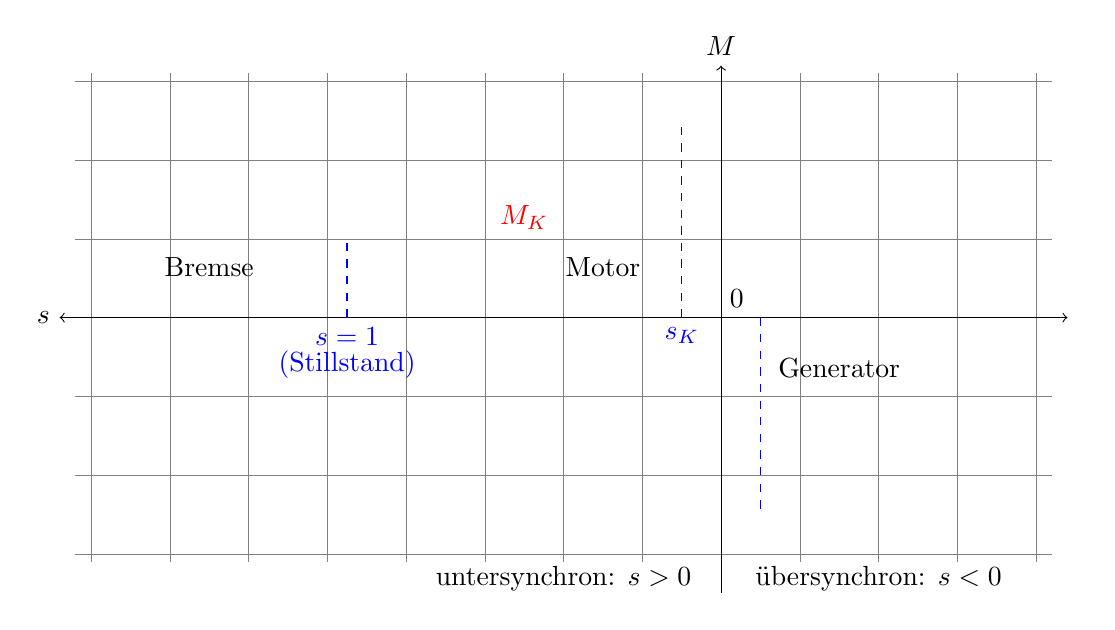
\begin{tikzpicture}[domain=-16:8, samples=200]
				\draw[very thin,color=gray] (-8.2,-3.1) grid (4.2,3.1);
				\draw[<->] (-8.4,0) node[left] {$s$} -- (4.4,0) node[right] {$\varPhi$};
				\draw[->] (0,-3.5) -- (0,3.2) node[above] {$M$};
				\draw[color=red, scale=1/2, smooth] plot[id=klossche_kennlinie] function{-5 * (2 / (x / 0.96 + 0.96 / x))} node[right] {};
				\draw (0.2,0) node[above] {$0$};
				\draw[color=red] (-2.5,1) node[above] {$M_K$};
				\draw[dashed, color=blue] (-0.5,0) node[below] {${s_K}$} -- (-0.5,2.5);
				\draw[dashed, color=blue] (0.5,0) node[above] {} -- (0.5,-2.5);
				\draw[dashed, color=blue] (-4.75,0) node[below] {${s = 1}$} -- (-4.75,1);
				\draw[color=blue] (-4.75,-0.3) node[below] {(Stillstand)};
				\draw (-6.5,0.4) node[above] {Bremse};
				\draw (-1.5,0.4) node[above] {Motor};
				\draw (1.5,-0.4) node[below] {Generator};
				\draw (-2,-3.6) node[above] {untersynchron: $s > 0$};
				\draw (2,-3.6) node[above] {übersynchron: $s < 0$};
				\end{tikzpicture}
				}{{\bf Klossche Kennlinie.} Drehzahl/Drehmomenten-Kennlinie einer Asynchronmaschine. \label{kloss}}
		}
		\b{
			\fu{
				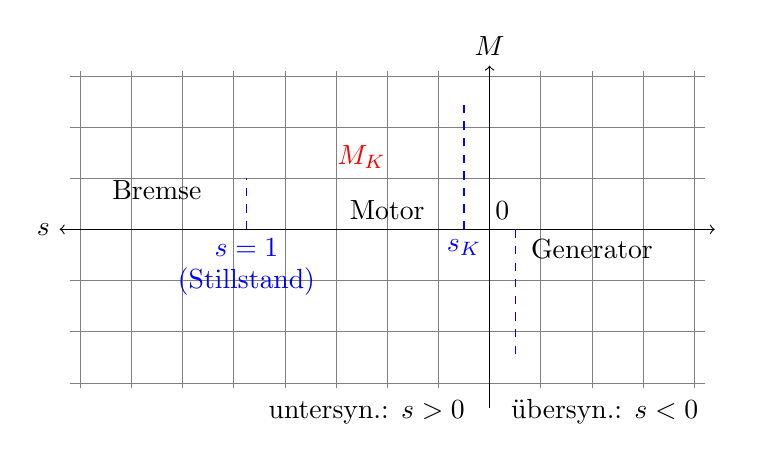
\begin{tikzpicture}[domain=-16:8, samples=200,  scale=0.65]
				\draw[very thin,color=gray] (-8.2,-3.1) grid (4.2,3.1);
				\draw[<->] (-8.4,0) node[left] {$s$} -- (4.4,0) node[right] {$\varPhi$};
				\draw[->] (0,-3.5) -- (0,3.2) node[above] {$M$};
				\draw[color=red, scale=1/2, smooth] plot[id=klossche_kennlinie] function{-5 * (2 / (x / 0.96 + 0.96 / x))} node[right] {};
				\draw (0.25,0) node[above] {$0$};
				\draw[color=red] (-2.5,1) node[above] {$M_K$};
				\draw[dashed, color=blue] (-0.5,0) node[below] {${s_K}$} -- (-0.5,2.5);
				\draw[dashed, color=blue] (0.5,0) node[above] {} -- (0.5,-2.5);
				\draw[dashed, color=blue] (-4.75,0) node[below] {${s = 1}$} -- (-4.75,1);
				\draw[color=blue] (-4.75,-0.55) node[below] {(Stillstand)};
				\draw (-6.5,0.4) node[above] {Bremse};
				\draw (-2,0) node[above] {Motor};
				\draw (2,0) node[below] {Generator};
				\draw (-2.4,-4) node[above] {untersyn.: $s > 0$};
				\draw (2.25,-4) node[above] {übersyn.: $s < 0$};
				\end{tikzpicture}
				}{Klossche Kennlinie}
		}

	\end{columns}
\end{frame}


\begin{frame}\ftx{Beispiel: Asynchronmaschine}
	\begin{bsp}{Asynchronmaschine}{}
		Ein Drehstrom-Asynchronmotor hat die folgenden Typenschildangaben:
		\begin{columns}
			\column[c]{0.5\textwidth}
				\begin{itemize}
					\item Nennleistung: $10\,$kW
					\item Nenndrehzahl: $1440\,\frac{\mathrm{U}}{\mathrm{min}}$
				\end{itemize}
			\column[c]{0.5\textwidth}
				\begin{itemize}
					\item Frequenz: $50\,$Hz
					\item Kippschlupf: 25\%
				\end{itemize}
		\end{columns}\b{\vspace{0.3cm}}
		Berechnen Sie das Nennmoment, das Kippmoment und das Anlaufmoment.
		\s{
			\begin{align*}
				P_\mathrm{N} &= M_\mathrm{N}\cdot \omega_\mathrm{N} = M_\mathrm{N}\cdot 2\pi n_\mathrm{N}\\
				M_\mathrm{N} &= \frac{P_\mathrm{N}}{2\pi n_\mathrm{N}} = \frac{10\cdot 10^3\,\mathrm{W}}{2\pi\cdot 1440 \frac{1}{60\,\mathrm{s}}} = 66,31\,\mathrm{Nm}\\
				s_\mathrm{N} &= \frac{\omega_\mathrm{s} - \omega_\mathrm{r}}{\omega_\mathrm{s}}\\
				&=\frac{2\pi \cdot 1500 \,\frac{1}{60\,\mathrm{s}} - 2\pi\cdot 1440\,\frac{1}{60\,\mathrm{s}}}{2\pi \cdot 1500 \,\frac{1}{60\,\mathrm{s}}}\\
				& = 0,04
			\end{align*}
			Für die Berechnung der weiteren Momente wird Gleichung \ref{GlKloss} für die Fälle Nennbetrieb und Stillstand ausgerechnet.
			\begin{align*}
				M &= \frac{2\cdot M_\mathrm{K}}{\frac{s_\mathrm{K}}{s} + \frac{s}{s_\mathrm{K}}}\\
				M_\mathrm{K} &= \frac{M_\mathrm{N}}{2}\cdot\left(\frac{s_\mathrm{K}}{s_\mathrm{N}} + \frac{s_\mathrm{N}}{s_\mathrm{K}}\right)\\
				&= \frac{66,31\,\mathrm{Nm}}{2}\cdot\left(\!\frac{0,25}{0,04} + \frac{0,04}{0,25}\!\right) = 212,54\,\mathrm{Nm}\\
				M_\mathrm{A} &= \frac{2\cdot 212,54\,\mathrm{Nm}}{\frac{0,25}{1} + \frac{1}{0,25}} = 100,02\,\mathrm{Nm}
			\end{align*}
		}
		\b{
		\only<2-3>{
				\begin{align*}
					\uncover<2->{P_\mathrm{N} &= M_\mathrm{N}\cdot \omega_\mathrm{N} = M_\mathrm{N}\cdot 2\pi n_\mathrm{N}}\\
					\uncover<2->{M_\mathrm{N} &= \frac{P_\mathrm{N}}{2\pi n_\mathrm{N}} = \frac{10\cdot 10^3\,\mathrm{W}}{2\pi\cdot 1440 \frac{1}{60\,\mathrm{s}}} = 66,31\,\mathrm{Nm}}\\
					\uncover<3->{s_\mathrm{N} &= \frac{\omega_\mathrm{s} - \omega_\mathrm{r}}{\omega_\mathrm{s}}}\\
					\uncover<3->{&=\frac{2\pi \cdot 1500 \,\frac{1}{60\,\mathrm{s}} - 2\pi\cdot 1440\,\frac{1}{60\,\mathrm{s}}}{2\pi \cdot 1500 \,\frac{1}{60\,\mathrm{s}}}}\\
					\uncover<3->{& = 0,04}
					\onslide<1->
				\end{align*}
		}
		\only<4-5>{
				\begin{align*}
					\uncover<4->{M &= \frac{2\cdot M_\mathrm{K}}{\frac{s_\mathrm{K}}{s} + \frac{s}{s_\mathrm{K}}}}\\
					\uncover<4->{M_\mathrm{K} &= \frac{M_\mathrm{N}}{2}\cdot\left(\frac{s_\mathrm{K}}{s_\mathrm{N}} + \frac{s_\mathrm{N}}{s_\mathrm{K}}\right)}\\
					\uncover<4->{&= \frac{66,31\,\mathrm{Nm}}{2}\cdot\left(\!\frac{0,25}{0,04} + \frac{0,04}{0,25}\!\right) = 212,54\,\mathrm{Nm}}\\
					\uncover<5->{M_\mathrm{A} &= \frac{2\cdot 212,54\,\mathrm{Nm}}{\frac{0,25}{1} + \frac{1}{0,25}} = 100,02\,\mathrm{Nm} }
					\onslide<1->
				\end{align*}
		}
		}
	\end{bsp}
\end{frame}